\section{Manuel d'utilisation}

Cette application débute avec une boîte de dialogue qui laisse le choix entre deux rôles : Maître de Jeu (MJ) ou Joueur. Si "MJ" est choisi, l'application se met en tant que serveur pour accueillir les joueurs. Si "Joueur" est choisi, un assistant ce connexion apparaît pour choisir à quel serveur se connecter. \\

L'interface qui se présente comporte un Chat, un gestionnaire de tours et le lanceur de dés. Le Chat contient la liste des utilisateurs et permet aux joueurs et au MJ de communiquer. De plus, le chat possède des commandes qui s'introduisent par un /. Les commandes implémentées sont :

\begin{description}
	\item[/help] \hfill \\
		Affiche l'ensemble des autres commandes disponibles du chat avec les indications d'utilisation.
	\item[/nickname <pseudo>] \hfill \\
		Modifie le pseudo par celui qui suit la commande.
	\item[/roll <nombre de dés>d<valeur max du dé>] \hfill \\
		Roule un nombre de fois voulu du dé choisi. Peut s'utiliser en chuchotement.
	\item[/whisper <utilisateur> <message>] \hfill \\
		Envoie un message privé au joueur indiqué.
\end{description}

\begin{figure}[h!]
	\centering
	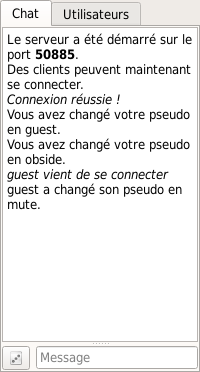
\includegraphics[scale=0.5]{img/chat_mj.png}
	\hspace{10 mm}
	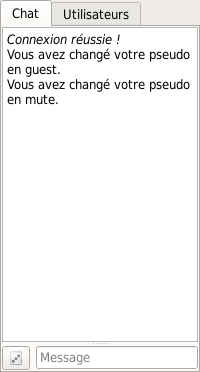
\includegraphics[scale=0.5]{img/chat_player.png}
	\caption{Chat MJ (à gauche) et chat Joueur (à droite)}
\end{figure}

Le Chat propose également une liste d'utilisateurs connectés. Un clic droit sur un ou plusieurs utilisateurs de cette liste affiche un menu contextuel donnant accès à des actions : Envoyer un message, et Lancer les dés.
La première action prépare un message privé à un ou plusieurs utilisateurs, la seconde lance les dés sélectionnés dans le lanceur de dés et envoie le résultat aux utilisateurs sélectionnés.


\begin{figure}[h!]
	\centering
	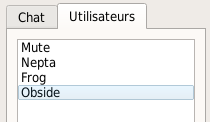
\includegraphics[scale=0.5]{img/chat_userlist_1.png}
	\hspace{10 mm}
	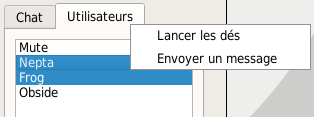
\includegraphics[scale=0.5]{img/chat_userlist_2.png}
	\caption{Liste d'utilisateurs (à gauche) et menu contextuel proposant des actions sur les utilisateurs sélectionnés (à droite)}
\end{figure}

Le lanceur de dés propose les dés les plus utilisés et permet de choisir pour chaque type de dé, le nombre de fois que celui-ci doit être lancé. Initialement, les compteurs sont à zéro. Pour augmenter le nombre de fois que l'on lance un dé, il faut appuyer sur le bouton correspondant ou utiliser la molette de la souris pour faire varier le nombre en étant sur le bouton. On peut ensuite décider de lancer les dés sur le chat (lancé public) ou de lancer les dés en privé si le MJ l'exige (lancé caché). Il est possible de réinitialiser tous les compteurs.

\begin{figure}[h!]
	\centering
	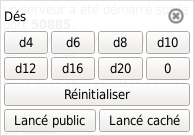
\includegraphics[scale=0.5]{img/dice_manager.png}
	\caption{Lanceur de dés}
\end{figure}

Le gestionnaire de tours est un outil qui permet au MJ de gérer ses combats. Il peut ajouter les joueurs ou personnages non joueurs (PNJ) en écrivant dans le champ de texte prévu à cet effet. Lorsque des utilisateurs se connectent, ils sont automatiquement ajoutés dans le gestionnaire de tour. Le MJ peut réordonner les tours à sa guise et dispose d'un certain nombre d'outils. Il peut ajouter des personnages comme dit précédemment, retirer un personnage à l'aide d'un bouton, déplacer les personnages dans le gestionnaire à la souris. Il dispose également de raccourcis clavier, par exemple les flèches du clavier permettent de naviguer entre les tours et de les réarranger.

\begin{figure}[h!]
	\centering
	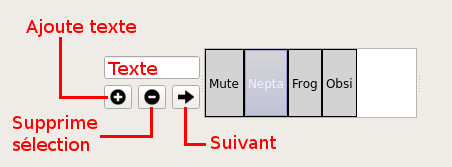
\includegraphics[scale=0.7]{img/turn_manager.jpg}
	\caption{Gestionnaire de tour}
\end{figure}